\section{Results}
\label{sec:results}

Table~\ref{tab:main} (Appendix~\ref{app:extra}) gives every RAMDocs condition, Table~\ref{tab:cb} every ConflictBank and RAGuard one, and
Table~\ref{tab:risk} splits answers into correct, misinformation and abstention. Every pre-registered test is listed,
by family, in the hypothesis tables of Appendix~\ref{app:extra}.

\subsection{A neutral flag changes whether the model answers, not what it answers}
\label{sec:neutral}
\begin{table*}[t]
\centering\small
\setlength{\tabcolsep}{3.5pt}
\resizebox{\textwidth}{!}{%
\begin{tabular}{lrrrrrrrrrrrr}
\toprule
& \multicolumn{4}{c}{No flags} & \multicolumn{4}{c}{Oracle, neutral flag} & \multicolumn{4}{c}{Oracle, directional flag} \\
\cmidrule(lr){2-5}\cmidrule(lr){6-9}\cmidrule(lr){10-13}
Generator & Correct & Misinfo. & Abstain & Sel. & Correct & Misinfo. & Abstain & Sel. & Correct & Misinfo. & Abstain & Sel. \\
\midrule
\multicolumn{13}{l}{\emph{RAMDocs, multi-answer prompt}} \\
gpt-4o-mini & 22.1 & 47.7 & 3.4 & 22.8 & 15.3 & \textbf{61.9} & 5.0 & 16.2 & 35.5 & \textbf{14.9} & 2.9 & \textbf{36.5} \\
gpt-6-luna & 14.4 & 72.2 & 1.2 & 14.6 & 11.3 & 76.7 & 0.7 & 11.4 & 53.5 & \textbf{11.3} & 1.4 & \textbf{54.3} \\
Claude Haiku 5.5 & 25.2 & 55.2 & 2.2 & 25.7 & 26.4 & \textbf{47.2} & 2.2 & 27.0 & 53.5 & \textbf{6.7} & 2.9 & \textbf{55.1} \\
gpt-6.1-terra & 10.8 & 75.5 & 2.2 & 11.0 & 10.1 & 81.3 & 1.4 & 10.2 & 50.4 & \textbf{13.7} & 2.2 & \textbf{51.5} \\
Claude Sonnet 5.5 & 45.3 & 24.5 & 2.2 & 46.3 & 45.3 & 21.6 & 2.2 & 46.3 & 59.7 & \textbf{3.6} & 1.4 & \textbf{60.6} \\
\midrule
\multicolumn{13}{l}{\emph{ConflictBank, multi-answer prompt}} \\
gpt-4o-mini & 21.6 & 72.8 & 0.3 & 21.6 & 12.8 & \textbf{83.2} & 0.9 & \textbf{12.9} & 49.4 & \textbf{41.2} & 1.2 & \textbf{50.1} \\
gpt-4.1 & 13.0 & 82.7 & 0.7 & 13.1 & 6.7 & \textbf{90.7} & 0.3 & \textbf{6.7} & 36.0 & \textbf{58.3} & 1.0 & \textbf{36.4} \\
Qwen2.5-7B & 23.7 & 67.0 & 6.0 & 25.2 & 15.3 & \textbf{79.0} & 5.0 & \textbf{16.1} & 41.3 & \textbf{52.0} & 13.0 & \textbf{47.5} \\
\midrule
\multicolumn{13}{l}{\emph{ConflictBank, one-answer prompt}} \\
gpt-4o-mini & 51.1 & 31.0 & 6.7 & 54.8 & 32.4 & \textbf{17.7} & \textbf{41.0} & 55.0 & 81.2 & \textbf{4.2} & \textbf{2.1} & \textbf{83.0} \\
gpt-6-luna & 53.6 & 24.3 & 11.9 & 60.8 & 44.1 & \textbf{17.4} & \textbf{28.9} & 62.0 & 90.0 & \textbf{0.0} & \textbf{0.8} & \textbf{90.7} \\
Claude Haiku 5.5 & 66.8 & 22.0 & 1.2 & 67.6 & 67.4 & 22.1 & 0.9 & 68.0 & 90.1 & \textbf{0.2} & 1.1 & \textbf{91.1} \\
gpt-6.1-terra & 73.0 & 18.0 & 1.7 & 74.2 & 70.7 & 15.7 & 4.7 & 74.1 & 90.0 & \textbf{0.7} & 0.3 & \textbf{90.3} \\
Claude Sonnet 5.5 & 75.7 & 15.7 & 1.0 & 76.4 & 78.7 & 12.0 & 1.7 & 80.0 & 92.0 & 1.0 & 1.7 & 93.6 \\
gpt-4.1 & 64.7 & 27.3 & 1.7 & 65.8 & 56.7 & 21.7 & 14.0 & 65.9 & 91.3 & 0.3 & 1.7 & 92.9 \\
Qwen2.5-7B & 50.3 & 35.3 & 5.0 & 53.0 & 47.0 & 28.7 & 15.0 & 55.3 & 75.7 & 13.0 & 1.3 & 76.7 \\
\midrule
\multicolumn{13}{l}{\emph{ConflictBank, forced choice}} \\
gpt-4o-mini & 55.4 & 31.6 & 0.1 & 55.5 & 55.2 & 31.9 & 0.4 & 55.5 & 79.7 & \textbf{6.7} & 0.0 & \textbf{79.7} \\
gpt-6-luna & 64.6 & 25.8 & 0.0 & 64.6 & 66.1 & 22.0 & 0.0 & 66.1 & 91.0 & \textbf{0.1} & 0.0 & \textbf{91.0} \\
Claude Haiku 5.5 & 69.3 & 20.9 & 0.0 & 69.3 & 73.2 & \textbf{16.8} & 0.0 & \textbf{73.2} & 90.4 & \textbf{0.0} & 0.0 & \textbf{90.4} \\
gpt-6.1-terra & 77.7 & 14.7 & 0.0 & 77.7 & 77.3 & 13.3 & 0.0 & 77.3 & 92.3 & \textbf{0.3} & 0.0 & \textbf{92.3} \\
\bottomrule
\end{tabular}}
\caption{Risk and coverage on conflict questions (\%): strictly correct answers, answers that contain the
misinformation, abstentions (``unknown''), and selective accuracy (correct answers over non-abstained answers, pooled
over questions and seeds). \textbf{Bold}: the change from no flags is significant (H21 for
ConflictBank one-answer and forced; the paper's exploratory family elsewhere). The answer policy decides what a neutral
flag does: under a prompt that asks for every valid answer it adds the misinformation to the answer; under a one-answer
prompt that allows ``unknown'' it moves answers, misinformed and correct, into abstention; under forced choice it has
no abstention to trade.}
\label{tab:risk}
\end{table*}


Flagging exactly the gold contradictions in the neutral format lowers gpt-4o-mini's RAMDocs conflict-question accuracy
by \adOracleFlagConf\ points \dOracleFlagConfCI\ from \plainConf\% (H2), and gpt-4.1's by \agptOracleFlagConf\ (H9).
On ConflictBank, even with a prompt stating that the question has one answer, it costs gpt-4o-mini
\azSgMiniOracleFlagConflict\ points and gpt-6-luna \azSgLunaOracleFlagConflict\ (H15, H19). Pooled over all
\nNeutralSettings\ settings (benchmarks, generators, prompts) with a random-effects model, the effect is
\neuPooled\ points \neuPooledCI\ ($\tau=\neuPooledTau$; settings share questions, so the interval is optimistic); \nNeutralHarm\ settings are significantly harmed and \nNeutralHelp\ helped (gpt-6-luna under majority
misinformation, Claude Haiku under the forced prompt). No Claude model is helped
(H25: Haiku \hTwentyFiveSgHaikuFlag, Sonnet \hTwentyFiveSgSonnetFlag\ on ConflictBank), and no generator on RAGuard
(H26; \hTwentySixRgLunaFlag\ to \hTwentySixRgSonnetFlag, none significant).

\paragraph{The mechanism is abstention.} Table~\ref{tab:risk} shows where the lost answers go. With the one-answer
prompt, gpt-4o-mini's neutral flag lowers the share of answers containing the misinformation by
\ahTwentyOneSgMiniFlagMisinfo\ points, but only by abstaining (\hTwentyOneSgMiniFlagAbstain\ points); its accuracy on
the questions it still answers is unchanged (\hTwentyOneSgMiniFlagSelective; H21). When ``unknown'' is not allowed
(the forced prompt, H20), the neutral flag has no effect on gpt-4o-mini (\hTwentyFcMiniFlag), gpt-6-luna
(\hTwentyFcLunaFlag) or gpt-6.1-terra (\hTwentyFcTerraFlag), and a small one on Claude Haiku (\hTwentyFcHaikuFlag).
Under the multi-answer prompt the flag instead makes the model list both sides (Figure~\ref{fig:answers}). The
answer policy decides how the model hedges; the directional flag cuts misinformation further while raising accuracy.

\paragraph{What the flag lacks is direction.} A flag that says one side of each pair is false, without which,
lowers gpt-4o-mini's ConflictBank accuracy by \azSgMiniOracleFlagOnewrongConflict\ points (H16). It helps only where
the other passages reveal which side is false: on RAMDocs, where several correct passages usually agree, it gains
gpt-6.1-terra \zRdTerraOracleFlagOnewrongConflict\ points, but on ConflictBank, one passage against one,
\zSgTerraOracleFlagOnewrongConflict. The pair structure does not leak direction: removing it from the one-wrong flag
raises RAMDocs accuracy (H22: \hTwentyTwoRdMiniOwNp\ with gpt-4o-mini, \hTwentyTwoRdLunaOwNp\ with gpt-6-luna). Given an
instruction to drop unreliable passages, adding the flag still costs \ahThirteenXMini\ points on RAMDocs and
\ahThirteenXCb\ on ConflictBank (H13). Asking the model to commit to the better-supported side (\emph{pick}) helps
the reasoning models (\zSgLunaOracleFlagPickConflict\ for gpt-6-luna on ConflictBank; exploratory). On
WikiContradict, where both sides are valid, the neutral flag \emph{raises} the share of answers giving both by
\awikiOracleFlag\ points \wikiOracleFlagCI\ (H8).

\subsection{Naming the false side is what helps}
\label{sec:direction}
\begin{table*}[t]
\centering\small
\setlength{\tabcolsep}{3.6pt}
\resizebox{\textwidth}{!}{%
\begin{tabular}{llrrrrrrrrrrr}
\toprule
& & & \multicolumn{2}{c}{Accuracy} & \multicolumn{4}{c}{Oracle pairs} & \multicolumn{2}{c}{LLM detector} & Single & LLM dir. \\
\cmidrule(lr){4-5}\cmidrule(lr){6-9}\cmidrule(lr){10-11}
Generator & Prompt & Seeds & Closed & Plain & Flag & One wrong & Dir.\ flag & Remove & Flag & Dir.\ flag & call & clean q. \\
\midrule
gpt-4o-mini & single & 3 & 10.0 & 51.1 & \textbf{$-$18.7} & \textbf{$-$35.7} & \textbf{$+$30.1} & \textbf{$+$35.0} & \textbf{$-$18.2} & $+$8.4 & $+$7.6 & $-$4.7 \\
gpt-4o-mini & multi & 3 & -- & 21.6 & \textbf{$-$8.8} & -- & \textbf{$+$27.9} & \textbf{$+$66.4} & \textbf{$-$8.4} & \textbf{$+$20.0} & -- & $-$1.0 \\
gpt-4o-mini & minimal & 3 & -- & 35.0 & \textbf{$-$18.1} & -- & \textbf{$+$38.4} & \textbf{$+$51.2} & -- & -- & -- & -- \\
gpt-4.1 & single & 1 & 20.0 & 64.7 & \textbf{$-$8.0} & \textbf{$-$35.3} & \textbf{$+$26.7} & \textbf{$+$26.0} & -- & $-$2.3 & -- & $-$3.0 \\
gpt-4.1 & multi & 1 & -- & 13.0 & \textbf{$-$6.3} & -- & \textbf{$+$23.0} & \textbf{$+$78.3} & \textbf{$-$6.7} & \textbf{$+$17.0} & -- & 0.0 \\
Qwen2.5-7B & single & 1 & 4.3 & 50.3 & $-$3.3 & $-$5.0 & \textbf{$+$25.3} & \textbf{$+$35.7} & $-$4.0 & $+$7.3 & -- & $-$1.0 \\
Qwen2.5-7B & multi & 1 & -- & 23.7 & \textbf{$-$8.3} & -- & \textbf{$+$17.7} & \textbf{$+$63.7} & $-$8.3 & $+$6.7 & -- & $-$1.0 \\
gpt-6-luna & single & 3 & 16.9 & 53.6 & \textbf{$-$9.4} & \textbf{$-$29.1} & \textbf{$+$36.4} & \textbf{$+$37.0} & \textbf{$-$9.3} & $+$8.6 & $-$6.3 & $-$1.3 \\
gpt-6.1-terra & single & 1 & 20.0 & 73.0 & $-$2.3 & $-$5.3 & \textbf{$+$17.0} & \textbf{$+$18.3} & $-$2.7 & \textbf{$-$11.7} & \textbf{$-$21.0} & 0.0 \\
\midrule
\multicolumn{13}{l}{\emph{Majority misinformation: three wrong-side passages, one correct}} \\
gpt-4o-mini & single & 3 & -- & 21.6 & $+$1.1 & -- & \textbf{$+$32.7} & \textbf{$+$65.1} & $-$2.2 & \textbf{$+$5.7} & $+$6.8 & $-$4.7 \\
gpt-6-luna & single & 3 & -- & 29.8 & \textbf{$+$6.6} & -- & \textbf{$+$60.4} & -- & -- & \textbf{$+$7.1} & -- & $-$1.3 \\
gpt-6.1-terra & single & 1 & -- & 26.0 & $-$3.7 & -- & \textbf{$+$66.3} & -- & -- & \textbf{$+$9.0} & -- & 0.0 \\
\bottomrule
\end{tabular}}
\caption{ConflictBank conflict questions (300; one correct answer each): accuracy (\%, one-way strict) closed-book
and with the passages but no flags, then the paired difference in points made by each format. \emph{Prompt}: the
answer policy: \emph{single} says there is one answer, \emph{multi} asks for every valid answer (our default
skeleton), \emph{minimal} states no policy. \emph{One wrong}: the neutral flag plus ``exactly one of the two
contains misinformation''. \emph{Single call}: one call that names the suspect passages, then answers. Last column:
the LLM directional flag's change on the 100 clean questions. The LLM detector is gpt-4o-mini for every generator.
\textbf{Bold}: significant under the paper's single scheme.}
\label{tab:cb}
\end{table*}

With the same oracle pairs, the directional flag beats the neutral and one-wrong flags in every setting we ran (H3,
H9--H12, H15, H16, H19, H25, H26). On ConflictBank it gains between
\azSgTerraOracleFlagDirectionalConflict\ and \azSgLunaOracleFlagDirectionalConflict\ points for the OpenAI generators,
\zSgHaikuOracleFlagDirectionalConflict\ for Claude Haiku and \zSgSonnetOracleFlagDirectionalConflict\ for Claude
Sonnet. It gains under the forced prompt (H20: \hTwentyFcTerraDir\ to \hTwentyFcLunaDir), when the misinformation
outnumbers the truth three to one (\zMjMiniOracleFlagDirectionalConflict\ to \zMjTerraOracleFlagDirectionalConflict;
Claude Haiku \hTwentyFiveMjHaikuDir), and on RAGuard's real posts (H26: \hTwentySixRgTerraDir\ to
\hTwentySixRgSonnetDir, all significant). On RAMDocs it gains \adOracleDirConf\ points with gpt-4o-mini and up to
\azRdTerraOracleFlagDirectionalConflict\ with gpt-6.1-terra, but not significantly for Qwen2.5-7B (Table~\ref{tab:generality}). It raises accuracy on answered questions by
\hTwentyOneSgTerraDirSelective\ to \hTwentyOneSgLunaDirSelective\ points (H21): unlike the neutral flag, it changes
which side the model picks.

On RAGuard every generator is less accurate with the posts than closed-book (gpt-4o-mini \zpRgMiniConflict\%
against \zcRgMiniConflict\%), as \citet{zeng2025raguard} report, mostly because the stronger models abstain
(gpt-6-luna on \zmRgLunaPlainUnknown\%); the flag removes misinformation answers but not this abstention.

\paragraph{Direction works like an answer key.} Telling the model ``the answer $X$ is false'', without marking any
passage, does about as well as the directional flag: none of the nine registered comparisons differs significantly (H23;
e.g.\ \hTwentyThreeSgMiniKey\ on ConflictBank and \hTwentyThreeRdMiniKey\ on RAMDocs for gpt-4o-mini). The oracle rows
are therefore upper bounds on what any detector can deliver, and the value of a flag lies in its direction. A wrong
direction is as strong a lever the other way: an inverted oracle that names the correct side costs \aadvDirConf\
points on RAMDocs and \azCbMiniOracleInvFlagDirectionalConflict\ on ConflictBank (exploratory).

\subsection{With real detectors, wrong-side flags are the cost}
\label{sec:real}
\begin{figure}[t]
\centering
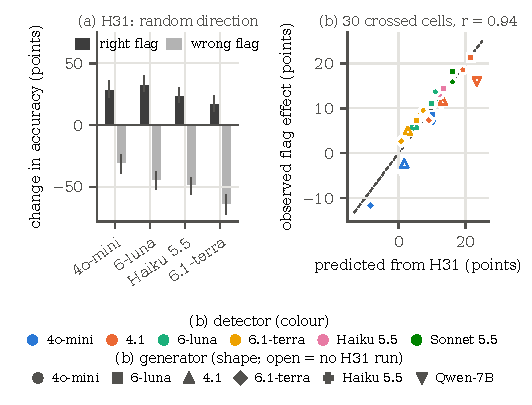
\includegraphics[width=\columnwidth]{generated/fig_reliability.pdf}
\caption{Each point is a detector--generator cell (ConflictBank, one-answer prompt, 300 conflict questions; bars:
95\% CIs). Left: the registered predictor, the detector's direction accuracy minus the generator's no-flag accuracy.
Right: the exploratory score, which credits right flags only where the generator errs and charges wrong-side flags
only where it is right. Table~\ref{tab:cells} lists the cells.}
\label{fig:reliability}
\end{figure}
A real detector's directional flag replaces the generator's judgement with the detector's, so it should pay only when
the detector's is better. H24 tests this on a common scale across \hTwentyFourCells\ crossed cells
(Figure~\ref{fig:reliability}): the gain rises with the detector's direction accuracy minus the generator's no-flag
accuracy ($\rho=\hTwentyFourRho$, $p\hTwentyFourP$; within cells, \hTwentyFourSlope\ points of gain per point of gap,
\hTwentyFourSlopeCI). It holds on the cells registered before Claude was added ($\rho=\hTwentyFourSthirteenRho$,
$p=\hTwentyFourSthirteenP$) and is weaker under majority misinformation ($\rho=\hTwentyFourMajRho$,
$p=\hTwentyFourMajP$; exploratory), where the gpt-4o-mini detector's direction falls to \cbmajDirAccLlm\%.

Yet the gain is positive in \hTwentyFourPos\ of \hTwentyFourCells\ cells, including many where the detector is less
accurate than the generator, so ``the detector must beat the generator'' is too strong. An exploratory, post-hoc
accounting explains why. A flag can help only where the generator would be wrong, and hurt only where it would be
right, so we credit the detector for naming the false side on the first kind of question and charge it for marking a
correct passage on the second. This score predicts the cell gains far better than the gap ($\rho=\hTwentyFourMechRho$;
Pearson $r=\hTwentyFourMechR$ against $\hTwentyFourGapR$). The gpt-4o-mini detector flags almost every question (\detAnyFlagMini\%) and
marks a correct passage as suspect on \detWrongDirMini\% of them: it helps the weaker generators (gpt-4o-mini
\zSgMiniLlmDirFlagDirectionalConflict, Qwen2.5-7B \zSgQwenLlmDirFlagDirectionalConflict) and lowers the accuracy of
the four most accurate (gpt-6.1-terra \zSgTerraLlmDirFlagDirectionalConflict; also Claude Sonnet, Claude Haiku and gpt-4.1). gpt-6.1-terra as a detector flags only
\detAnyFlagTerra\% of questions and marks a correct passage on \detWrongDirTerra\%; it names the false side less often
than gpt-4o-mini does, yet lowers no generator's accuracy. On RAGuard the same detector helps the Claude generators (H26: Haiku \hTwentySixRgHaikuLlm, Sonnet
\hTwentySixRgSonnetLlm) but not gpt-4o-mini (\hTwentySixRgMiniLlm).

\paragraph{Against published methods (H14) and a single call (H18).} Astute RAG \citep{wang2025astute} and TrustRAG
\citep{zhou2025trustrag} lose legitimate same-name answers on RAMDocs (gold recall \recMultiPlain\% to
\recMultiAst\% and \recMultiTr\%), and on ConflictBank they do not beat the one-answer prompt (\zSgMiniAstuteConflict\ and \zSgMiniTrustragConflict\ points; exploratory). A single call that
names the suspect passages before answering does not differ significantly from the gpt-4o-mini detector pipeline, at
half the calls (H18; equivalence within $\pm$3 points is not established), but
the reasoning models and Claude Haiku, asked to judge ConflictBank's generated passages, distrust most of them and
abstain, losing up to \azSgTerraSelfIdentifyClean\ points on clean questions. Table~\ref{tab:baselines}
(Appendix~\ref{app:more}) gives all baselines.

\subsection{What a detector must get right}
\label{sec:grid}
In synthetic detectors the gain rises with direction accuracy, and precision matters mainly for removal, whose false
flags delete correct passages (H4a); the grid predicts real detectors' effects only roughly (H6).
Appendix~\ref{app:grid} gives the cells and tests.
